\documentclass[12pt]{article}

% Language setting
\usepackage[english]{babel}

% Set page size and margins - A4 for European standard
\usepackage[a4paper,top=2.5cm,bottom=2.5cm,left=3cm,right=3cm,marginparwidth=1.75cm]{geometry}

% Useful packages
\usepackage{amsmath}
\usepackage{graphicx}
\usepackage[table]{xcolor}
\usepackage{csquotes}
\usepackage[colorlinks=true, allcolors=blue]{hyperref}
\usepackage{enumitem}
\usepackage{float}
\usepackage{caption}
\usepackage{subcaption}
\usepackage{tikz}
\usetikzlibrary{positioning,shadows}
\usepackage{pgfplots}
\pgfplotsset{compat=1.18}
\usepackage{booktabs}
\usepackage{multirow}
\usepackage{longtable}

% Bibliography - APA style as required
\usepackage[
backend=biber,
style=apa,
]{biblatex}

\addbibresource{sample.bib}

\begin{document}

% ---------------------------
% Title page (custom)
% ---------------------------
\begin{titlepage}
  \begin{center}
    \includegraphics[width=5cm]{nup_logo.png} \\[1cm]
    {\Large Neapolis University Pafos} \\[0.5cm]

    \begin{tabular}{@{}l@{}}
      {\large \textbf{Course Code:} IS506-EN\_F25} \\[0.2cm]
      {\large \textbf{Course Title:} Digital Innovation and Entrepreneurship} \\[0.2cm]
      {\large \textbf{Lecturer:} Marilia Kountouridou}
    \end{tabular} \\[2cm]

    {\huge \textbf{Development of a Digital Entrepreneurship Plan}} \\[0.5cm]
    {\Large \textbf{TerraSync:} Digital Twin Platform for Infrastructure \& Resource Optimization} \\[1.5cm]

     \begin{tabular}{@{}l@{}}
      {\large \textbf{Name:} Aleksandr Petrunin} \\[0.3cm]
      {\large \textbf{Student ID:} 1251114137}
    \end{tabular} \\[2cm]

    {\large \today}
  \end{center}
\end{titlepage}


% ---------------------------
% Table of Contents
% ---------------------------
\tableofcontents
\newpage

% ---------------------------
% 1. EXECUTIVE SUMMARY
% ---------------------------
\section{Executive Summary}

% Concise overview of the digital venture (150-200 words)
% - Problem statement
% - Solution overview
% - Target market
% - Unique value proposition
% - Business model highlights
% - Key financial projections


\textit{[Placeholder: Provide a compelling 150-200 word overview of TerraSync AI, highlighting the infrastructure optimization problem, your multimodal AI digital twin solution, target markets (Cyprus, Balkans, small EU economies), unique value proposition of n8n-orchestrated data integration, and key business metrics.]}

\newpage

% ---------------------------
% 2. STRATEGIC DIRECTION
% ---------------------------
\section{Strategic Direction}

\subsection{Vision Statement}
% Long-term aspirational goal
To become the leading territory-wide digital twin platform empowering sustainable infrastructure development across emerging economies worldwide.

\subsection{Mission Statement}
% Purpose and how you achieve the vision
We orchestrate scattered data sources into actionable intelligence, enabling governments and enterprises to reduce resource waste, accelerate sustainable development, and make data-driven infrastructure decisions.

\subsection{Strategic Goals and Objectives}
% 3-5 SMART goals aligned with digital strategy

\paragraph{Goal 1: Market entry and product validation:}
Within six months of launch, secure one pilot project with a Cyprus government ministry by integrating at least five core data sources and delivering one validated use case (e.g., port efficiency), leveraging existing partnerships and alignment with EU Cohesion Fund requirements to demonstrate product–market fit in the public sector.

\paragraph{Goal 2: Technology development:}
Build and deploy a robust, scalable data integration and analytics capability that delivers prediction accuracy of at least 75\% within twelve months of launch, enabling reliable infrastructure optimization insights across multiple territories and reducing decision-making time by 50\%.

\paragraph{Goal 3: Revenue targets:}
Achieve €1.5 million in annual recurring revenue by the end of Year 2 through a diversified customer base of at least three government entities and two enterprise clients, establishing sustainable growth and positive unit economics that support long-term profitability.

\paragraph{Goal 4: Geographic expansion:}
Expand operational presence to six additional territories across the Balkans and Baltic regions by the end of Year 2, increasing territory coverage from 9,251 sq km to at least 50,000 sq km, while maintaining consistent service quality and customer success outcomes.

\paragraph{Goal 5: Customer satisfaction and retention:}
Achieve and maintain a customer retention rate of 95\% and net customer satisfaction score of 8.5/10 by Year 2, building long-term strategic partnerships through exceptional customer success and continuous product improvement aligned with customer needs.


\subsection{Key Performance Indicators (KPIs)}

\begin{table}[H]
\centering
\caption{Strategic KPIs and Targets}
\begin{tabular}{@{}lllll@{}}
\toprule
\textbf{KPI} & \textbf{Baseline} & \textbf{Year 1} & \textbf{Year 2} & \textbf{Year 3} \\ \midrule
Customer Acquisition (Governments) & 0 & 1 & 3 & 6 \\
Data Sources Integrated & 0 & 5 & 15 & 30 \\
Annual Recurring Revenue (€) & 0 & 500K & 1.5M & 4M \\
Territory Coverage (sq km) & 0 & 9,251 & 50,000 & 150,000 \\
Prediction Accuracy (\%) & -- & 75 & 85 & 92 \\
Customer Retention Rate (\%) & -- & 70 & 95 & 98 \\
Customer Satisfaction Score (1-10) & -- & 7.0 & 8.5 & 9.0 \\
\bottomrule
\end{tabular}
\end{table}

\newpage

% ---------------------------
% 3. MARKET & ENVIRONMENTAL ANALYSIS
% ---------------------------
\section{Market \& Environmental Analysis}

\subsection{Market Overview and Opportunity}

\subsubsection{Target Market Definition}
% Define your target market segments

\subparagraph{Primary Market:} EU governments and ministries in small-to-medium economies (Cyprus, Balkans, Baltic states) responsible for infrastructure planning, sustainability compliance, and resource management.

\subparagraph{Secondary Market:} Large construction and engineering firms operating in these regions requiring project optimization and EU Green Deal compliance.

\subparagraph{Market Size:}
\begin{itemize}
    \item Global digital twin market: \$17.73B (2024) → \$259.32B (2032) at 40.1\% CAGR \cite{fortunebi2025digitaltwin}
    \item Infrastructure investment needed globally: \$57 trillion by 2030 \cite{mckinseyinfrastructure2020}
    \item EU Cohesion Fund allocation: 37\% directed to climate objectives across 15 eligible countries \cite{eucommission2021cohesionfund}
\end{itemize}

\subsubsection{TAM, SAM, SOM Analysis}

\begin{itemize}
    \item \textbf{TAM (Total Addressable Market): €16.4 Billion (\$17.7B)}
    \begin{itemize}
        \item \textit{Definition:} Global Digital Twin Market (2024 baseline) \cite{fortunebi2025digitaltwin}.
        \item \textit{Growth:} Projected to reach €240B by 2032 (40.1\% CAGR).
        \item \textit{Relevance:} Represents the theoretical ceiling for TerraSync if the platform expands globally across all industrial sectors and geographies.
    \end{itemize}

    \item \textbf{SAM (Serviceable Available Market): €1.2 Billion}
    \begin{itemize}
        \item \textit{Definition:} Digital Infrastructure \& GovTech market in EU Cohesion Fund eligible countries (15 nations including Cyprus, Greece, Baltics, and CEE region).
        \item \textit{Calculation:} Estimated as $\sim$7\% of the Global Digital Twin market, adjusted for the specific economic size of the target regions and the high intensity of EU-funded infrastructure development.
        \item \textit{Driver:} €392B EU Cohesion Policy (2021-2027), with significant allocations for digital and green transition projects \cite{eucommission2021cohesionfund}.
    \end{itemize}

    \item \textbf{SOM (Serviceable Obtainable Market): €50 Million}
    \begin{itemize}
        \item \textit{Definition:} Immediate capture potential within 3-5 years targeting Government Ministries and Tier-1 Construction firms in primary markets.
        \item \textit{Calculation (Bottom-Up):}
        \begin{itemize}
            \item \textbf{Public Sector:} 15 Countries $\times$ 4 Key Ministries $\times$ €500K avg. contract value = €30M.
            \item \textbf{Private Sector:} 200 Major Projects $\times$ €100K avg. license = €20M.
        \end{itemize}
        \item \textit{Target:} Capturing 8\% of this SOM (€4M ARR) by Year 3 is the primary strategic objective.
    \end{itemize}
\end{itemize}

\subsubsection{Industry Trends and Drivers}
\begin{enumerate}
    \item \textbf{EU Green Deal Mandates:} The European Climate Law legally binds member states to reduce net greenhouse gas emissions by at least 55\% by 2030, creating urgent demand for carbon monitoring tools. \cite{europeanparliament2024greendeal}.
    \item \textbf{Digital Twin Adoption:} The global market is expanding at a 40\%+ CAGR as industries shift from static models to dynamic, real-time simulations powered by IoT and AI. \cite{fortunebi2025digitaltwin}.
    \item \textbf{Infrastructure Crisis:} Systemic inefficiencies result in projects running 20\% over schedule and 80\% over budget, necessitating digital solutions for resource management. \cite{mckinsey2016construction}.
    \item \textbf{Data Integration Demand:} Smart city initiatives are hindered by fragmented data silos, creating a critical need for platforms that can orchestrate information across diverse departments. \cite{OECD2020}.
    \item \textbf{EU Funding Availability:} The 2021-2027 Cohesion Policy and EIB lending priorities specifically allocate capital to support the digital and green transition in less developed EU regions. \cite{EUCohesion2021, EIB2023}.
\end{enumerate}

\subsection{SWOT Analysis}

\begin{table}[H]
\centering
\caption{SWOT Analysis for TerraSync}
\begin{tabular}{@{}p{0.45\textwidth}p{0.45\textwidth}@{}}
\toprule
\textbf{Strengths} & \textbf{Weaknesses} \\ \midrule
\begin{itemize}[leftmargin=*, nosep]
    \item Modular, self-hosted architecture ensuring data sovereignty
    \item High extensibility via user-defined data adapters
    \item Agnostic to data types (integrates any user-managed source)
    \item Aligned with EU sustainability mandates
    \item Scalable core with community-driven extension ecosystem
\end{itemize} &
\begin{itemize}[leftmargin=*, nosep]
    \item Reliance on client technical capability for custom adapters
    \item Lack of pre-built integrations for legacy government systems
    \item Dependency on quality of user-provided data
    \item Small initial team vs. enterprise support networks
    \item Complexity in visualizing heterogeneous data sources
\end{itemize} \\ \midrule
\textbf{Opportunities} & \textbf{Threats} \\ \midrule
\begin{itemize}[leftmargin=*, nosep]
    \item Growing EU Green Deal compliance needs
    \item 40\% CAGR digital twin market
    \item EU funding for target regions
    \item Lack of territory-wide solutions
    \item Network effects from shared extension library
\end{itemize} &
\begin{itemize}[leftmargin=*, nosep]
    \item Established players (Siemens, Bentley) pivoting to open ecosystems
    \item Long government procurement cycles favoring established vendors
    \item Regulatory changes in data sovereignty/AI liability
    \item Resistance to open/modular systems in public sector
    \item Economic downturns reducing innovation budgets
\end{itemize} \\ \bottomrule
\end{tabular}
\end{table}

\subsection{PESTEL Analysis}

\begin{table}[H]
\centering
\caption{PESTEL Analysis for TerraSync}
\begin{tabular}{@{}p{0.15\textwidth}p{0.8\textwidth}@{}}
\toprule
\textbf{Factor} & \textbf{Implications} \\ \midrule
\textbf{Political} & 
\begin{itemize}[leftmargin=*, nosep]
    \item EU accession requirements for Balkans create infrastructure investment pressure
    \item Government stability varies across target markets
    \item Public procurement regulations favor transparency and competition
\end{itemize} \\ \midrule
\textbf{Economic} & 
\begin{itemize}[leftmargin=*, nosep]
    \item Target markets have GNI < 90\% EU average, qualifying for Cohesion Fund support
    \item Infrastructure spending is countercyclical (stimulus during downturns)
    \item Cost savings (20-30\% waste reduction) highly attractive given budget constraints
\end{itemize} \\ \midrule
\textbf{Social} & 
\begin{itemize}[leftmargin=*, nosep]
    \item Growing public demand for sustainability and transparency
    \item Urbanization driving smart city initiatives
    \item Skilled labor shortages in construction sector
    \item Cultural integration and peace-building through shared cross-border infrastructure
\end{itemize} \\ \midrule
\textbf{Technological} & 
\begin{itemize}[leftmargin=*, nosep]
    \item Rapid advancement in IoT sensors and satellite imagery (cost reduction)
    \item AI/ML models improving prediction accuracy
    \item Cloud computing enabling scalable infrastructure
    \item 5G networks enabling real-time data transmission
\end{itemize} \\ \midrule
\textbf{Environmental} & 
\begin{itemize}[leftmargin=*, nosep]
    \item Climate change increasing extreme weather events (need for resilience planning)
    \item Resource scarcity driving efficiency requirements
    \item EU Green Deal creating regulatory mandates
\end{itemize} \\ \midrule
\textbf{Legal} & 
\begin{itemize}[leftmargin=*, nosep]
    \item GDPR compliance required for data handling
    \item Data sovereignty concerns
    \item Public procurement laws
    \item Liability frameworks for AI-driven decisions
\end{itemize} \\ \bottomrule
\end{tabular}
\end{table}

\subsection{Competitive Analysis}

\subsubsection{Direct Competitors}
\begin{table}[H]
\centering
\caption{Competitive Landscape Analysis}
\small
\begin{tabular}{@{}p{0.15\textwidth}p{0.2\textwidth}p{0.25\textwidth}p{0.25\textwidth}@{}}
\toprule
\textbf{Competitor} & \textbf{Offering} & \textbf{Strengths} & \textbf{Weaknesses} \\ \midrule
\href{https://www.bentley.com/}{Bentley Systems} & iTwin platform & Established brand, BIM integration & Project-focused, not territory-wide \\
\href{https://insights-hub.siemens.com/}{Siemens} & MindSphere (Insights Hub) & Industrial IoT expertise & Complex, expensive, steep learning curve \\
\href{https://construction.autodesk.com/}{Autodesk} & Construction Cloud & Design tool integration & Limited predictive analytics, vendor lock-in \\
\href{https://www.3ds.com/3dexperience}{Dassault Systèmes} & 3DEXPERIENCE & Simulation capabilities & High cost, requires specialized expertise \\
\href{https://qgis.org}{QGIS} / \href{https://www.blender.org}{Blender} & Open Source Tools & Free, flexible, community-driven & Fragmented workflows, requires manual integration \\ \bottomrule
\end{tabular}
\end{table}

\textbf{Our Differentiation Strategy: The "Open Integrator" Advantage}

Unlike established competitors who build "walled gardens" optimized for their proprietary data formats, TerraSync positions itself as a vendor-agnostic orchestration layer.
\begin{itemize}
    \item \textbf{Data Sovereignty \& Self-Hosting:} We offer full on-premise or private cloud deployment options, addressing the strict data residency requirements of government clients that SaaS-only competitors often fail to meet.
    \item \textbf{Modular Extensibility:} Rather than relying on a fixed menu of integrations, our architecture allows local IT teams and the open-source community to build custom data adapters for legacy or niche government systems.
    \item \textbf{Vendor-Agnostic Aggregation:} We do not prioritize any specific CAD/BIM format. TerraSync acts as a neutral "glue" layer, visualizing data from Autodesk, Siemens, and local Excel sheets side-by-side without forcing data migration.
    \item \textbf{Cost Structure Alignment:} By leveraging existing open-source tools for the core, our pricing model is based on value (territory coverage) rather than user seats, aligning better with public sector budget structures.
\end{itemize}

\begin{figure}[H]
\centering
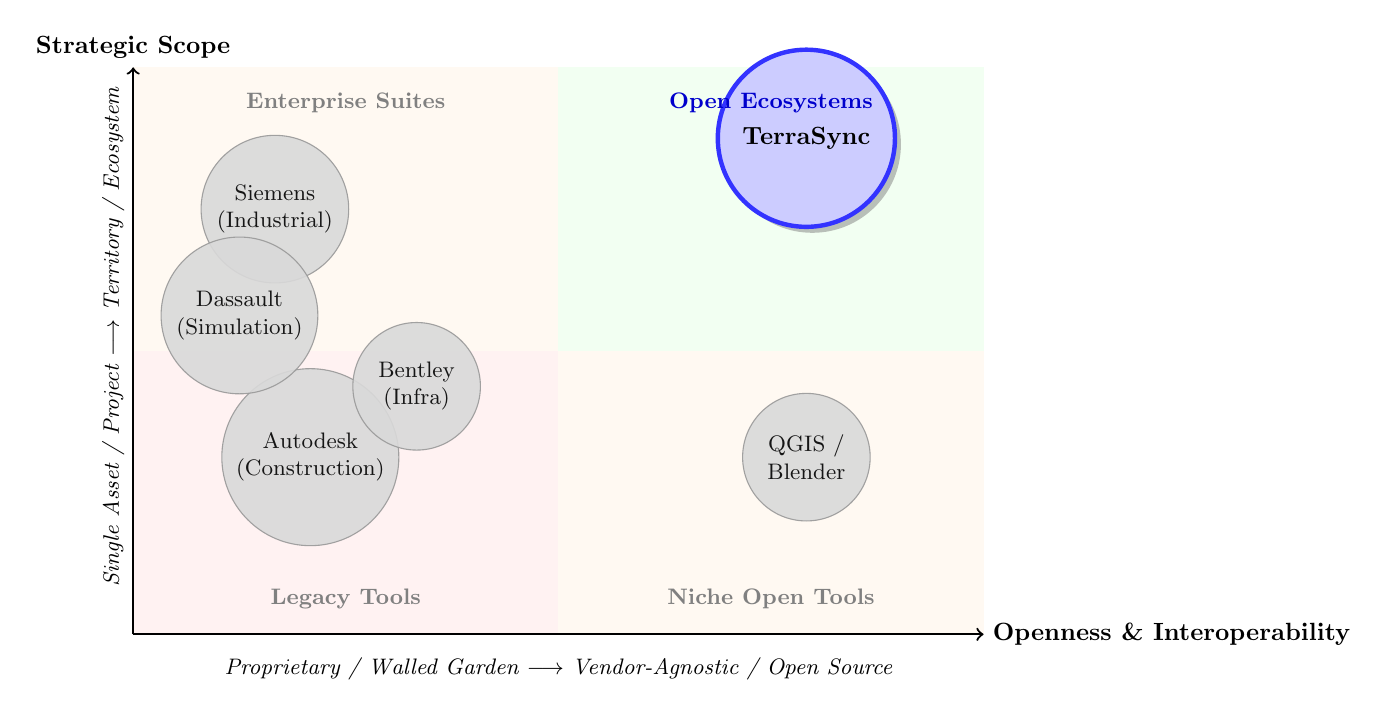
\begin{tikzpicture}[scale=0.9, transform shape]
    % Define coordinates
    \coordinate (O) at (0,0);
    \coordinate (X) at (12,0);
    \coordinate (Y) at (0,8);

    % Background quadrants
    \fill[red!5] (0,0) rectangle (6,4);
    \fill[orange!5] (0,4) rectangle (6,8);
    \fill[orange!5] (6,0) rectangle (12,4);
    \fill[green!5] (6,4) rectangle (12,8);

    % Draw Axes
    \draw[->, thick] (O) -- (X) node[right] {\textbf{Openness \& Interoperability}};
    \draw[->, thick] (O) -- (Y) node[above] {\textbf{Strategic Scope}};

    % Axis descriptions
    \node[below=0.2cm, font=\small\itshape] at (6,0) {Proprietary / Walled Garden $\longrightarrow$ Vendor-Agnostic / Open Source};
    \node[rotate=90, above=0.2cm, font=\small\itshape] at (0,4) {Single Asset / Project $\longrightarrow$ Territory / Ecosystem};

    % Competitor Nodes
    \node[circle, fill=gray!30, draw=gray!80, align=center, font=\small, minimum size=1.8cm, opacity=0.9] at (2.5, 2.5) {Autodesk\\(Construction)};
    \node[circle, fill=gray!30, draw=gray!80, align=center, font=\small, minimum size=1.8cm, opacity=0.9] at (4.0, 3.5) {Bentley\\(Infra)};
    \node[circle, fill=gray!30, draw=gray!80, align=center, font=\small, minimum size=1.8cm, opacity=0.9] at (2.0, 6.0) {Siemens\\(Industrial)};
    \node[circle, fill=gray!30, draw=gray!80, align=center, font=\small, minimum size=1.8cm, opacity=0.9] at (9.5, 2.5) {QGIS /\\Blender};
    \node[circle, fill=gray!30, draw=gray!80, align=center, font=\small, minimum size=1.8cm, opacity=0.9] at (1.5, 4.5) {Dassault\\(Simulation)};

    % TerraSync Node
    \node[circle, fill=blue!20, draw=blue!80, ultra thick, align=center, font=\bfseries, minimum size=2.5cm, drop shadow] at (9.5, 7.0) {TerraSync};

    % Quadrant Labels
    \node[font=\bfseries\small, gray] at (3, 7.5) {Enterprise Suites};
    \node[font=\bfseries\small, gray] at (3, 0.5) {Legacy Tools};
    \node[font=\bfseries\small, gray] at (9, 0.5) {Niche Open Tools};
    \node[font=\bfseries\small, blue!80!black] at (9, 7.5) {Open Ecosystems};

\end{tikzpicture}
\caption{Competitive Positioning Matrix: TerraSync occupies the high-value "Open Ecosystem" quadrant, differentiating from legacy "walled gardens".}
\label{fig:comp_matrix}
\end{figure}

\newpage

% ---------------------------
% 4. INNOVATION DESIGN
% ---------------------------
\section{Innovation Design}

\subsection{Problem Statement}

Infrastructure planning in emerging economies suffers from a "Digital Divide." While data exists, it is trapped in disconnected silos, making holistic decision-making impossible. Planners face three critical barriers:
\begin{itemize}
    \item \textbf{The "Walled Garden" Trap:} Enterprise digital twins (e.g., Siemens, Bentley) are prohibitively expensive and lock governments into proprietary formats.
    \item \textbf{The Visualization Gap:} Technical data (GIS, CAD) is unintelligible to non-technical stakeholders (ministers, public), leading to poor policy alignment.
    \item \textbf{Static Information:} Master plans are often outdated PDF snapshots rather than living models that react to real-time changes.
\end{itemize}

\subsection{Solution Overview: TerraSync Platform}

\subsubsection{Core Innovation}
TerraSync democratizes digital twin technology by fusing **Open Source Geospatial Intelligence (QGIS)** with **Cinematic Visualization (Blender)**. Instead of a black-box proprietary engine, we provide a transparent, modular platform that turns raw data into a "Living Territory Model."

\textbf{Key Innovation Elements:}
\begin{enumerate}
    \item \textbf{QGIS Integration Core:} Leverages the industry-standard open-source GIS engine for rigorous scientific accuracy and data layering.
    \item \textbf{Blender "Decision Theater":} Utilizes Blender not for daily operations, but for high-fidelity "what-if" simulations and public communication, bridging the gap between technical data and stakeholder understanding.
    \item \textbf{Low-Code Orchestration (n8n):} Acts as the platform's "nervous system," automatically pulling data from IoT sensors, weather APIs, and legacy databases without complex custom coding.
    \item \textbf{Explainable Decision Support Models:} Replaces "black-box" AI with transparent, rule-based and regression models (e.g., flood risk, congestion) that prioritize explainability for public sector accountability.
\end{enumerate}

\subsubsection{Technology Architecture}

\textit{[Placeholder: Insert system architecture diagram: Data Sources $\rightarrow$ n8n Hub $\rightarrow$ QGIS/PostGIS $\rightarrow$ Blender/Web Viewer]}

\textbf{1. The "Nervous System" (Ingestion \& Orchestration):}
\begin{itemize}
    \item \textbf{n8n Workflow Engine:} Automates the retrieval of data from diverse sources (Weather APIs, IoT traffic sensors, Excel registries).
    \item \textbf{Apache Kafka:} Buffers high-velocity real-time streams before processing.
\end{itemize}

\textbf{2. The "Brain" (Processing \& Analytics):}
\begin{itemize}
    \item \textbf{QGIS + PostGIS:} The authoritative "state of truth." Handles coordinate systems, zoning laws, and infrastructure layers.
    \item \textbf{Explainable AI Modules:} Runs transparent decision support scripts:
    \begin{itemize}
        \item \textit{Flood Risk:} Hydrology models based on terrain and weather data.
        \item \textit{Congestion:} Historical regression analysis of traffic patterns.
        \item \textit{Resource Bottlenecks:} Rule-based constraint logic.
    \end{itemize}
\end{itemize}

\textbf{3. The "Face" (Visualization \& Interaction):}
\begin{itemize}
    \item \textbf{CesiumJS / WebGL (Operational View):} Delivers a lightweight, interactive version of the twin via standard web browsers for daily monitoring.
    \item \textbf{Blender 3D (Strategic View):} Generates cinematic "Digital Twin" assets for major policy presentations and complex scenario simulations.
\end{itemize}

\textbf{Key Benefits:}
\begin{itemize}
    \item \textbf{Demonstrated Efficiency:} Potential to reduce infrastructure waste by up to 25\% through predictive optimization.
    \item \textbf{Rapid Time-to-Value:} Deploy initial pilots in weeks rather than years, enabling iterative feedback loops.
    \item \textbf{EU Green Deal Compliance:} Automated sustainability reporting aligned with EU mandates.
    \item \textbf{Data Sovereignty:} Full ownership of data and models, eliminating "black box" vendor risks.
    \item \textbf{Cost Effectiveness:} Significantly lower total cost of ownership compared to custom enterprise digital twins, with role-based access control (RBAC).
    \item \textbf{Open Standards:} All data exportable in non-proprietary formats (GeoJSON, IFC) to prevent vendor lock-in.
\end{itemize}

\subsubsection{Minimum Viable Product (MVP)}

The TerraSync MVP focuses on delivering immediate value through the Cyprus pilot while establishing the foundation for territorial expansion. This initial release prioritizes essential functionality over comprehensive features, enabling rapid deployment and iterative improvement based on real government feedback.

\paragraph{Core Features}
The MVP delivers territory-wide data integration through five essential n8n workflows connecting weather services, maritime traffic, infrastructure databases, and IoT sensor networks. Basic QGIS processing provides geospatial analysis with coordinate system normalization and data layer management. A simplified CesiumJS web interface enables government staff to monitor territory conditions without specialized training. Rule-based alerting triggers notifications for predefined thresholds like port congestion or weather warnings.

\paragraph{Initial Data Sources}
Five strategic data integrations establish the platform foundation. Cyprus Meteorological Service provides real-time weather data and forecasting through automated API connections. AIS maritime tracking delivers vessel positions and estimated arrival times for Limassol Port operations. OpenStreetMap and Cyprus cadastral databases supply authoritative geographic and infrastructure layers. Municipal databases contribute road network status, traffic patterns, and utility information. IoT sensor pilots in two locations provide proof-of-concept for environmental monitoring expansion.

\paragraph{Essential Visualization}
The MVP visualization balances functionality with development speed. CesiumJS web interface displays real-time territory data with basic 3D terrain and infrastructure overlays accessible through standard browsers. Interactive data layer toggles let users examine individual information sources or combined views. Time-series charts show historical trends and current conditions for key performance indicators. Basic Blender templates create static 3D renderings for stakeholder presentations, establishing the foundation for future "Decision Theater" capabilities.

\paragraph{n8n Workflow Library}
Five core workflows automate critical data processes without custom coding requirements. Weather data ingestion pulls meteorological information every hour, processes forecasts, and triggers alerts for extreme conditions. Port logistics monitoring correlates vessel arrivals with customs capacity to predict congestion patterns. Infrastructure status tracking monitors road closures, utility outages, and maintenance schedules from municipal systems. Environmental sensor integration collects IoT data from pilot locations and validates data quality. Stakeholder notification workflows deliver automated reports and alerts through email, SMS, and dashboard updates.

\paragraph{Cyprus Pilot Specifications}
The Cyprus deployment addresses immediate government planning needs while demonstrating scalability potential. Coverage spans the Limassol district including port operations, urban areas, and rural communities affected by seasonal tourism. Integration focuses on existing government IT systems including customs databases, municipal planning records, and emergency services communications.

\subsection{Value Proposition}

\textbf{For Government Ministries:}
\begin{itemize}
    \item Reduce infrastructure waste by 25\% through predictive optimization
    \item Achieve EU Green Deal compliance with automated sustainability reporting
    \item Make data-driven decisions with real-time territory intelligence
    \item Deploy in weeks (vs. 1-2 years for custom solutions)
    \item Pay fraction of cost compared to custom digital twin development
\end{itemize}

\textbf{For Construction Enterprises:}
\begin{itemize}
    \item Optimize resource allocation across multiple projects
    \item Reduce delays through predictive risk assessment
    \item Improve bid accuracy with better data
    \item Demonstrate sustainability compliance to clients
\end{itemize}

\subsection{Customer Journey and Use Cases}

\subsubsection{Use Case 1: Operational Efficiency – Smart Port Logistics (Limassol, Cyprus)}
\textbf{The Challenge:} Port authorities struggle with congestion due to disconnected data systems (maritime traffic, customs databases, weather forecasts), leading to truck idle times and increased emissions.
\textbf{The TerraSync Solution:}
\begin{itemize}
    \item \textbf{Ingestion:} n8n workflows pull real-time AIS ship tracking data and local weather API feeds.
    \item \textbf{Processing:} A rule-based AI model correlates incoming vessel volume with customs processing capacity.
    \item \textbf{Action:} The system triggers automated alerts to logistics companies via SMS/Email to stagger truck arrivals.
    \item \textbf{Visualization:} Operators view a live CesiumJS dashboard showing vessel positions and yard occupancy.
\end{itemize}
\textbf{Outcome:} Reduced truck idle time by 15\% and lowered port carbon emissions (Green Deal alignment).

\subsubsection{Use Case 2: Strategic Planning – Cross-Border Transport Corridor (Balkans)}
\textbf{The Challenge:} Planning a highway connecting Montenegro and Albania requires integrating incompatible GIS datasets from two nations and assessing environmental impact on protected areas.
\textbf{The TerraSync Solution:}
\begin{itemize}
    \item \textbf{Integration:} QGIS acts as the "Rosetta Stone," normalizing geospatial data from both countries into a single coordinate system.
    \item \textbf{Simulation:} Blender is used to create a photorealistic "Decision Theater" simulation of the proposed route, highlighting visual impact on tourism zones.
    \item \textbf{Consensus:} Ministers from both countries use the interactive 3D model during summits to agree on route adjustments in real-time.
\end{itemize}
\textbf{Outcome:} Accelerated planning approval by 6 months and secured EU Cohesion funding through transparent impact assessment.

\subsubsection{Use Case 3: Climate Resilience – Urban Flood Defense System}
\textbf{The Challenge:} A mid-sized municipality faces recurring flash floods but lacks the budget for enterprise-grade hydrological modeling software.
\textbf{The TerraSync Solution:}
\begin{itemize}
    \item \textbf{Sensing:} Low-cost IoT rain gauges are deployed in key catchment areas, connected via LoRaWAN.
    \item \textbf{Analysis:} An explainable hydrological model runs on the QGIS terrain layer, predicting runoff paths based on current rainfall intensity.
    \item \textbf{Response:} n8n triggers automated road closure warnings to municipal police and updates the public web map.
\end{itemize}
\textbf{Outcome:} Zero casualties during extreme weather events and reduced property damage claims.

\subsubsection{Use Case 4: Rural Sustainability – Forest Village Revitalization (Troodos Mountains, Cyprus)}
\textbf{The Challenge:} Traditional forest villages in the Troodos Mountains suffer from seasonal population decline and limited year-round economic activity, while facing increasing climate-related risks including wildfires and water scarcity. Government planners need comprehensive data to design infrastructure investments and policies that can revive these communities, attract sustainable tourism, and create year-round economic opportunities.
\textbf{The TerraSync Solution:}
\begin{itemize}
    \item \textbf{Environmental Risk Assessment:} IoT sensors monitor climate conditions including soil moisture, temperature, and humidity to help government planners understand wildfire patterns and water resource dynamics for informed infrastructure investment decisions.
    \item \textbf{Infrastructure Planning:} QGIS integrates dam capacity, road access, telecommunications coverage, and seasonal utility usage to identify optimal locations for government investment in broadband, renewable energy, and water management systems.
    \item \textbf{Economic Development Visualization:} Blender creates compelling 3D presentations showing potential development scenarios to attract private investment, showcase tourism opportunities, and demonstrate community revival possibilities to EU funding bodies.
    \item \textbf{Investment Impact Modeling:} Predictive analytics help government planners assess which infrastructure improvements will generate the highest economic return and community sustainability outcomes.
\end{itemize}
\textbf{Outcome:} Government gains data-driven insights to target €2M in EU rural development funding, leading to enhanced broadband infrastructure that enables remote work opportunities, sustainable tourism growth, and gradual community revitalization with 25\% increase in year-round residents.

\subsection{Innovation Feasibility and Evidence}

\textbf{Technical Feasibility:}
\begin{itemize}
    \item n8n: Open-source, proven workflow automation (100K+ installations)
    \item Digital twin technology: \$17.73B existing market with established vendors \cite{fortunebi2025digitaltwin}
    \item AI/ML: Pre-trained models available (Azure, AWS, open-source)
    \item Data availability: Public datasets + commercial partnerships
\end{itemize}

\textbf{Customer Validation:}
\begin{itemize}
    \item EU Cohesion Fund prioritizes digital infrastructure projects
    \item 15 EU countries eligible for funding in target market
    \item Growing demand: 40.1\% CAGR in digital twin adoption
\end{itemize}

\begin{figure}[H]
\centering
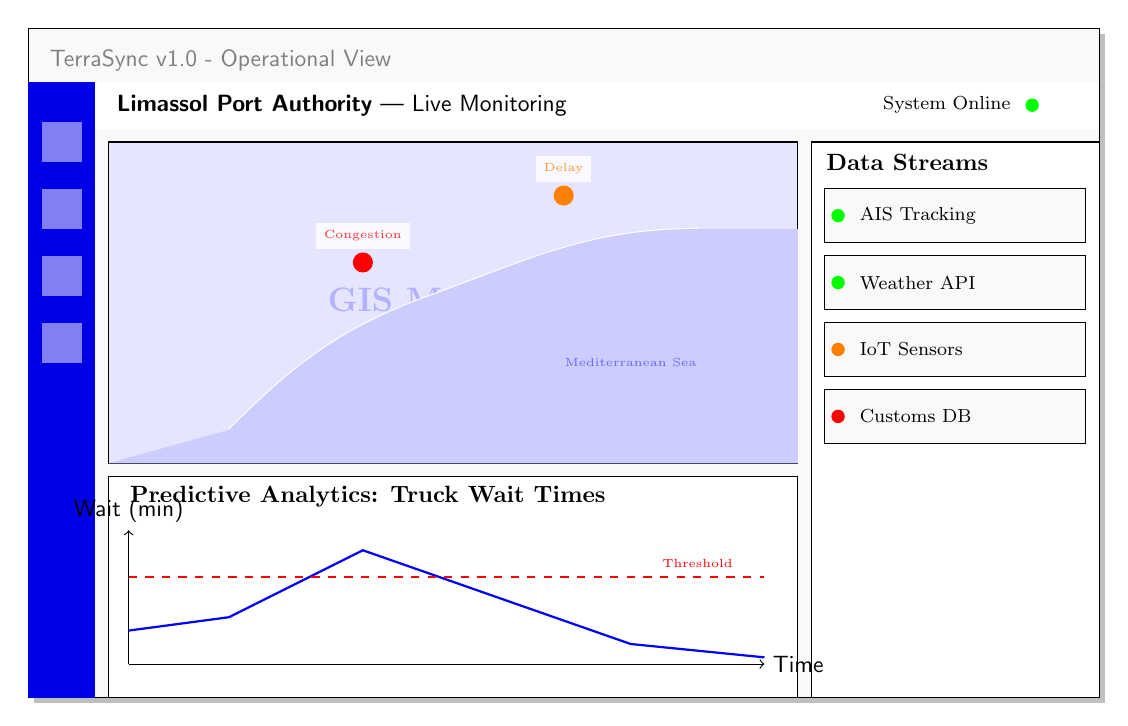
\begin{tikzpicture}[scale=0.85, transform shape, font=\sffamily]
    % Main Window
    \draw[fill=gray!5, drop shadow] (0,0) rectangle (16,10);
    \node[anchor=north west, text=gray] at (0.2,9.8) {TerraSync v1.0 - Operational View};

    % Sidebar
    \fill[blue!90!black] (0,0) rectangle (1,9.2);
    \foreach \y in {8,7,6,5} \fill[white, opacity=0.5] (0.2,\y) rectangle (0.8,\y+0.6);

    % Top Bar
    \fill[white] (1,8.5) rectangle (16,9.2);
    \node[anchor=west] at (1.2, 8.85) {\textbf{Limassol Port Authority} | Live Monitoring};
    \fill[green] (15, 8.85) circle (0.1);
    \node[anchor=east, font=\footnotesize] at (14.8, 8.85) {System Online};

    % Map Area
    \draw[fill=blue!10] (1.2, 3.5) rectangle (11.5, 8.3);
    \node[blue!30, font=\bfseries\Large] at (6.35, 5.9) {GIS Map View};
    % Map details
    \draw[white, thick] (3,4) to[out=45,in=200] (6,6) to[out=20,in=180] (10,7); % Coastline
    \fill[blue!20] (3,4) to[out=45,in=200] (6,6) to[out=20,in=180] (10,7) -- (11.5,7) -- (11.5,3.5) -- (1.2,3.5) -- cycle; % Sea
    \node[font=\tiny, text=blue!60] at (9, 5) {Mediterranean Sea};
    
    % Pins
    \fill[red] (5, 6.5) circle (0.15); \node[above, font=\tiny, fill=white, opacity=0.8, text=red] at (5, 6.7) {Congestion};
    \fill[orange] (8, 7.5) circle (0.15); \node[above, font=\tiny, fill=white, opacity=0.8, text=orange] at (8, 7.7) {Delay};

    % Right Panel - Data Feed
    \draw[fill=white] (11.7, 0) rectangle (16, 8.3);
    \node[anchor=west, font=\bfseries] at (11.8, 8.0) {Data Streams};
    
    % Stream Items
    \foreach \y/\t/\c in {6.8/AIS Tracking/green, 5.8/Weather API/green, 4.8/IoT Sensors/orange, 3.8/Customs DB/red} {
        \draw[fill=gray!5] (11.9, \y) rectangle (15.8, \y+0.8);
        \fill[\c] (12.1, \y+0.4) circle (0.1);
        \node[anchor=west, font=\footnotesize] at (12.3, \y+0.4) {\t};
    }

    % Bottom Panel - Analytics
    \draw[fill=white] (1.2, 0) rectangle (11.5, 3.3);
    \node[anchor=west, font=\bfseries] at (1.4, 3.0) {Predictive Analytics: Truck Wait Times};
    % Graph
    \draw[->] (1.5, 0.5) -- (11, 0.5) node[right] {Time};
    \draw[->] (1.5, 0.5) -- (1.5, 2.5) node[above] {Wait (min)};
    \draw[blue, thick] (1.5, 1) -- (3, 1.2) -- (5, 2.2) -- (7, 1.5) -- (9, 0.8) -- (11, 0.6);
    \draw[red, dashed] (1.5, 1.8) -- (11, 1.8);
    \node[red, font=\tiny] at (10, 2.0) {Threshold};

\end{tikzpicture}
\caption{Concept Wireframe: The TerraSync Operational Dashboard. The interface integrates real-time GIS visualization (center) with live n8n data streams (right) and predictive analytics (bottom) to support rapid decision-making.}
\label{fig:dashboard_wireframe}
\end{figure}

\newpage

% ---------------------------
% 5. DIGITAL BUSINESS MODEL
% ---------------------------
\section{Digital Business Model}

\subsection{Business Model Canvas}

\begin{figure}[H]
\centering
\resizebox{\textwidth}{!}{
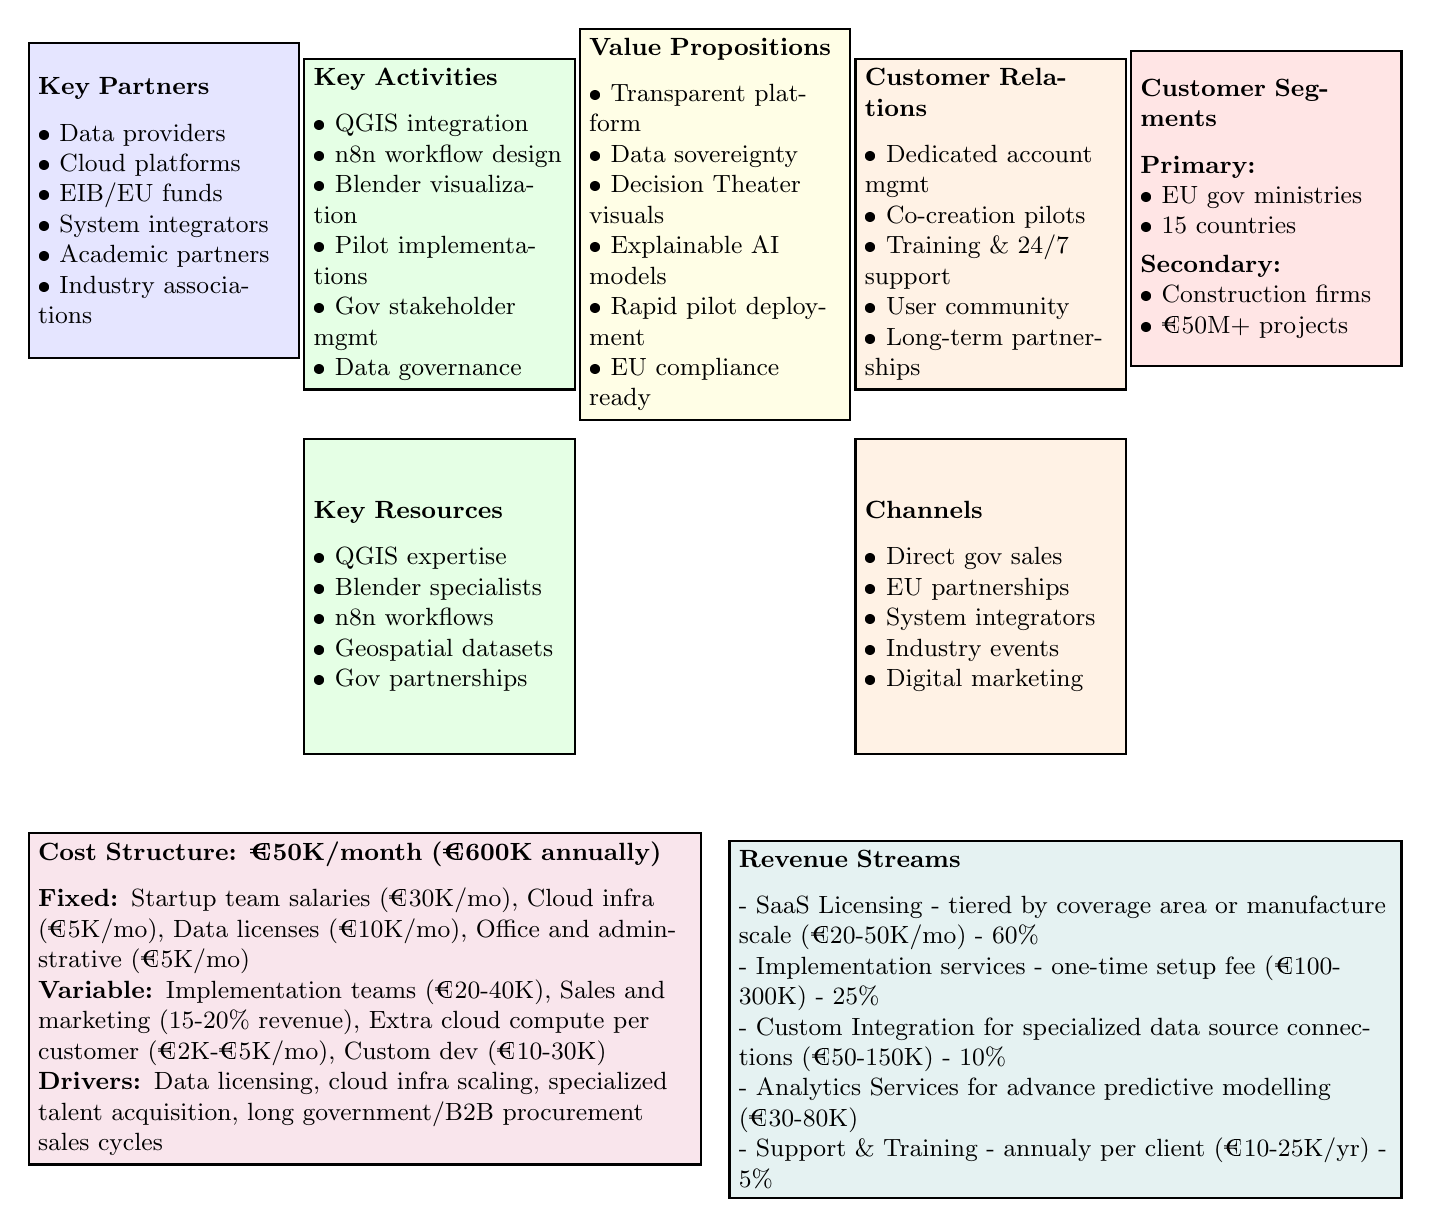
\begin{tikzpicture}[
    box/.style={rectangle, draw, thick, text width=3.2cm, minimum height=4cm, align=left, font=\small},
    tallbox/.style={rectangle, draw, thick, text width=3.2cm, minimum height=8.2cm, align=left, font=\small},
    widebox/.style={rectangle, draw, thick, text width=8.3cm, minimum height=4cm, align=left, font=\small},
    title/.style={font=\bfseries\small},
]

% Row 1 - Top boxes
\node[box, fill=blue!10] (kp) at (0,0.3) {
    \textbf{Key Partners}\\[0.2cm]
    • Data providers\\
    • Cloud platforms\\
    • EIB/EU funds\\
    • System integrators\\
    • Academic partners\\
    • Industry associations
};

\node[box, fill=green!10] (ka) at (3.5,0) {
    \textbf{Key Activities}\\[0.2cm]
    • QGIS integration\\
    • n8n workflow design\\
    • Blender visualization\\
    • Pilot implementations\\
    • Gov stakeholder mgmt\\
    • Data governance
};

\node[box, fill=yellow!10] (vp) at (7,0) {
    \textbf{Value Propositions}\\[0.2cm]
    • Transparent platform\\
    • Data sovereignty\\
    • Decision Theater visuals\\
    • Explainable AI models\\
    • Rapid pilot deployment\\
    • EU compliance ready
};

\node[box, fill=orange!10] (cr) at (10.5,0) {
    \textbf{Customer Relations}\\[0.2cm]
    • Dedicated account mgmt\\
    • Co-creation pilots\\
    • Training \& 24/7 support\\
    • User community\\
    • Long-term partnerships
};

\node[box, fill=red!10] (cs) at (14,0.2) {
    \textbf{Customer Segments}\\[0.2cm]
    \textbf{Primary:}\\
    • EU gov ministries\\
    • 15 countries\\[0.1cm]
    \textbf{Secondary:}\\
    • Construction firms\\
    • €50M+ projects
};

% Row 2 - Bottom boxes
\node[box, fill=green!10, below=0.6cm of ka] (kr) {
    \textbf{Key Resources}\\[0.2cm]
    • QGIS expertise\\
    • Blender specialists\\
    • n8n workflows\\
    • Geospatial datasets\\
    • Gov partnerships
};

\node[box, fill=orange!10, below=0.6cm of cr] (ch) {
    \textbf{Channels}\\[0.2cm]
    • Direct gov sales\\
    • EU partnerships\\
    • System integrators\\
    • Industry events\\
    • Digital marketing
};

% Row 3 - Wide bottom boxes
\node[widebox, fill=purple!10, below=6.0cm of kp.south west, anchor=north west] (cost) {
    \textbf{Cost Structure: €50K/month (€600K annually)}\\[0.2cm]
    \textbf{Fixed:} Startup team salaries (€30K/mo), Cloud infra (€5K/mo), Data licenses (€10K/mo), Office and adminstrative (€5K/mo)\\
    \textbf{Variable:} Implementation teams (€20-40K), Sales and marketing (15-20\% revenue), Extra cloud compute per customer (€2K-€5K/mo), Custom dev (€10-30K)\\
    \textbf{Drivers:} Data licensing, cloud infra scaling, specialized talent acquisition, long government/B2B procurement sales cycles
};

\node[widebox, fill=teal!10, below=6.0cm of cs.south east, anchor=north east] (revenue) {
    \textbf{Revenue Streams}\\[0.2cm]
    - SaaS Licensing - tiered by coverage area or manufacture scale (€20-50K/mo) - 60\%\\
    - Implementation services - one-time setup fee (€100-300K) - 25\%\\
    - Custom Integration for specialized data source connections (€50-150K) - 10\%\\
    - Analytics Services for advance predictive modelling (€30-80K)\\
    - Support \& Training - annualy per client (€10-25K/yr) - 5\%
};

\end{tikzpicture}
}
\caption{TerraSync AI Business Model Canvas}
\end{figure}

\subsubsection{Customer Segments}
\textbf{Primary segment:} EU Government Ministries responsible for infrastructure, transport, environment, and regional development in 15 countries with GNI below 90\% EU average, requiring EU Green Deal compliance and resource optimization tools.

\textbf{Secondary segment:} Large construction and engineering firms (€50M+ projects) operating in target regions, needing EU compliance documentation and project optimization capabilities.

\subsubsection{Value Propositions}
TerraSync delivers rapid pilot deployment through transparent, open-source components (QGIS, Blender) rather than proprietary black-box solutions. We provide data sovereignty through on-premise deployment options, explainable decision support models for public sector accountability, and cinematic "Decision Theater" visualizations that bridge the gap between technical data and stakeholder understanding. The platform enables EU Green Deal compliance tracking and scales from municipal pilots to cross-border initiatives in months.

\subsubsection{Channels}
We reach customers through direct government procurement processes, EU partnership programs including EIB financing packages and Cohesion Fund applications, strategic alliances with system integrators like Accenture and Deloitte, presence at EU infrastructure summits and smart city conferences, and targeted digital marketing via LinkedIn, industry publications, and published case studies.

\subsubsection{Customer Relationships}
We maintain dedicated account management for government clients, co-create solutions through pilot projects with early adopters, provide comprehensive training and support including on-site workshops, documentation, and 24/7 helpdesk services, foster user communities for best practice sharing, and establish long-term partnerships through multi-year contracts with expansion clauses.

\textbf{Projected Revenue Mix (Year 3):}
SaaS licensing accounts for 60\% of revenue, implementation services 25\%, custom integration and analytics 10\%, and support and training 5\%.

\subsubsection{Key Resources}
Our human capital includes QGIS specialists and geospatial analysts, Blender visualization artists, n8n workflow designers, and infrastructure domain experts with government experience. Intellectual assets comprise proprietary workflow templates for municipal operations, explainable AI model libraries, and our unique "Decision Theater" methodology. Physical resources encompass development infrastructure, demo environments, and partnership agreements with data providers (weather services, satellite imagery). Financial resources include €500K-1M seed funding and EIB co-investment arrangements.

\subsubsection{Key Activities}
Core activities include QGIS data integration and geospatial analysis, n8n workflow design and automation, Blender "Decision Theater" visualization development, explainable AI model development and validation, customer pilot implementations and stakeholder training, government relationship management and compliance documentation, and ongoing platform enhancement based on user feedback.

\subsubsection{Key Partnerships}
Strategic partnerships span the open-source ecosystem including QGIS and Blender community contributors; data providers such as weather services, Copernicus satellite imagery, and national statistical offices; technology infrastructure providers (cloud hosting, IoT sensor networks); funding partners including the European Investment Bank and EU Cohesion Fund administrators; implementation partners such as municipal consulting firms and local system integrators; and academic partners for geospatial research and model validation.

\newpage

% ---------------------------
% 6. DIGITAL TOOLS INTEGRATION
% ---------------------------
\section{Digital Tools Integration}

\subsection{Technology Stack Overview}

\begin{table}[H]
\centering
\caption{Comprehensive Technology Stack}
\small
\begin{tabular}{@{}p{0.2\textwidth}p{0.25\textwidth}p{0.2\textwidth}p{0.25\textwidth}@{}}
\toprule
\textbf{Category} & \textbf{Tool/Technology} & \textbf{Purpose} & \textbf{Rationale} \\ \midrule
Orchestration & n8n & Workflow automation & Open-source, auditable, low-code \\
GIS Processing & QGIS + PostGIS & Geospatial analysis & Industry standard, transparent \\
3D Visualization & Blender & Decision Theater & Cinematic quality, open-source \\
Web Visualization & CesiumJS + WebGL & Operational dashboards & Browser-native, real-time \\
Data Streaming & Apache Kafka & IoT sensor ingestion & Scalable, reliable \\
Explainable AI & Scikit-learn + SHAP & Decision support & Transparent, auditable models \\
Storage & PostGIS + TimescaleDB & Geospatial + time-series & Optimized for territory data \\
API Management & Kong Gateway & Service orchestration & Security, rate limiting \\
Monitoring & Prometheus + Grafana & System observability & Open-source, government-friendly \\
DevOps & Docker + Kubernetes & Container orchestration & Scalability, portability \\
\bottomrule
\end{tabular}
\end{table}

\subsection{Core Platform Components}

\subsubsection{n8n Orchestration Hub}
The n8n workflow automation platform acts as TerraSync's central nervous system. Its visual workflow design lets non-technical government staff create and modify data integrations without programming knowledge. With over 400 pre-built connectors for APIs, databases, and webhooks, the platform cuts integration complexity and supports custom Python and JavaScript code for specialized government needs.

The self-hosted deployment gives complete data sovereignty, meeting government concerns about data residency and control. The open-source foundation saves money compared to enterprise integration platforms that cost \$10K-50K monthly. Examples show the platform's versatility: weather data updates territory risk assessments and alerts stakeholders, satellite imagery feeds object detection models that create infrastructure change reports, and IoT sensor networks trigger predictive maintenance workflows with automatic work order generation.

\subsubsection{Explainable AI Pipeline}
TerraSync's AI approach puts transparency first over algorithmic complexity, recognizing that government stakeholders need to understand and justify automated decisions. The data preprocessing works directly in the QGIS environment for spatial accuracy as it cleans, normalizes, and combines multi-source datasets. Feature engineering extracts predictive variables from established geospatial layers, incorporating elevation models, proximity analyses, and land use classifications that government planners already understand and trust.

The platform uses transparent and auditable model types: rule-based decision trees for flood risk assessment, linear regression for traffic congestion prediction, constraint satisfaction algorithms for resource allocation, and Monte Carlo simulations for scenario planning. Each model type provides clear explanations, with SHAP values and decision tree visualizations meeting public sector accountability requirements. Government stakeholder review processes validate model acceptance before deployment, building trust through collaboration rather than imposed solutions.

\subsubsection{"Decision Theater" Visualization}
The platform uses two visualization approaches for different needs: strategic decision-making and operational monitoring. Blender's professional 3D engine creates high-quality cinematic presentations for stakeholder meetings, ministerial briefings, and public consultations where visual impact and clear narratives drive policy acceptance. The automated QGIS-to-Blender pipeline transforms complex geospatial datasets into accessible 3D scenes without manual modeling work.

For daily operations, CesiumJS provides lightweight, browser-based monitoring that government staff can access without specialized hardware or software. The platform supports dynamic scenario simulations for "what-if" visualizations in policy impact assessment, and real-time data layer toggling lets users examine infrastructure, environmental, and social data independently or together. Temporal controls enable historical event playback and future scenario simulation, supporting both retrospective analysis and forward-looking planning.

\subsection{Scalability and Performance}

The current TerraSync setup handles over one million data points daily and supports five to ten territories at once with sub-second dashboard response times. This baseline performance comes from careful optimization of the underlying PostGIS spatial database and efficient n8n workflow orchestration that minimizes computational overhead.

The scaling strategy uses Kubernetes horizontal auto-scaling to allocate computational resources based on demand for consistent performance during peak usage like emergency responses or major policy announcements. Global dashboard access uses content delivery networks to reduce delays for geographically distributed users, and database sharding by territory enables independent scaling of individual deployments. Multi-region cloud deployment provides backup and localized performance optimization, supporting the platform's expansion across diverse government jurisdictions with varying technical infrastructure.

\subsection{Security and Compliance}

Data security follows industry best practices with end-to-end encryption using TLS 1.3 protocols for data integrity during transmission between system components and external interfaces. Role-based access control provides detailed permission management, letting government administrators restrict data access by organizational hierarchies and job functions. Sensitive information gets automated anonymization when appropriate, and the platform maintains a SOC 2 Type II compliance roadmap for audit and certification requirements.

European GDPR compliance means the platform only collects and keeps data needed for operations. Citizens and organizations can request data removal through built-in erasure tools. Data Processing Agreements with external partners set clear rules about information sharing. EU data residency rules are met by keeping servers in Frankfurt and Dublin, so European data stays within proper jurisdictions.

\subsection{Integration Roadmap}

The three-phase development approach balances quick deployment with long-term growth, so government partners can see value fast and build toward comprehensive territorial intelligence systems.

Phase 1 establishes the TerraSync foundation during months one through six, implementing the core QGIS and PostGIS geospatial infrastructure alongside five essential n8n workflows connecting weather services, IoT networks, and government databases. Basic Blender visualization templates provide immediate stakeholder communication, and the Cyprus pilot deployment serves as proof-of-concept validation.

Phase 2 expands capabilities during months seven through twelve with advanced "Decision Theater" functionality that transforms stakeholder engagement through immersive visualization experiences. Integration scope increases to fifteen or more data sources and CesiumJS web interfaces enable daily operational monitoring by government staff. Multi-territory support extends platform utility across three countries, accompanied by an explainable AI model library that provides transparent decision support for diverse government applications.

Phase 3 achieves governance and scale objectives during year two through development of thirty government-certified data workflows that meet public sector audit and compliance standards. White-label municipal deployment packages enable rapid expansion across smaller government entities, and mobile applications provide field worker access to territorial intelligence. The open-source community ecosystem evolves into a collaborative workflow marketplace where government organizations can share integration patterns and analytical models, fostering innovation and reducing individual development costs.

\newpage

% ---------------------------
% 7. SCENARIO-BASED PLANNING
% ---------------------------
\section{Scenario-Based Planning}

\subsection{Scenario 1: Best Case - "Rapid Adoption"}

\paragraph{Key Assumptions}
The Cyprus pilot succeeds within 6 months, demonstrating clear value to government stakeholders. EU Green Deal enforcement accelerates, creating urgent demand for compliance tools. Two additional governments sign contracts by Month 12, driven by positive media coverage and compelling case studies from the Cyprus deployment.

\paragraph{Strategic Response}
Rapid success triggers accelerated hiring to 10 employees by Year 2, supporting expansion to 5 Balkan countries. The team raises Series A funding of \$5M to fuel growth and develops white-label products for faster market penetration.

\paragraph{Financial Projections}
Revenue grows aggressively: Year 1 reaches €800K, Year 2 hits €2.5M, and Year 3 achieves €6M. Break-even occurs at Month 14, establishing strong cash flow for continued expansion.

\subsection{Scenario 2: Most Likely - "Steady Growth"}

\paragraph{Key Assumptions}
The Cyprus pilot takes 9-12 months to complete, facing typical government implementation challenges. Long government sales cycles average 18 months, limiting acquisition to 1 new government client per year. Competition from established players creates pricing pressure and longer evaluation periods.

\paragraph{Strategic Response}
Focus narrows to 2-3 core markets for deeper penetration rather than broad expansion. Controlled team growth reaches 5-7 employees by Year 2, balancing capability with cash flow. EIB co-investment arrangements provide patient capital aligned with government procurement cycles, and a strong customer success function maximizes retention.

\paragraph{Financial Projections}
Revenue grows steadily: Year 1 generates €500K, Year 2 reaches €1.5M, and Year 3 achieves €4M. Break-even occurs at Month 18, providing a sustainable growth trajectory.

\subsection{Scenario 3: Worst Case - "Slow Traction"}

\paragraph{Key Assumptions}
The Cyprus pilot faces delays lasting 12-18 months due to bureaucratic hurdles and technical challenges. Economic recession triggers budget cuts across target markets, reducing infrastructure spending. Data access restrictions limit platform functionality, and governments require longer proof-of-concept periods before committing.

\paragraph{Strategic Response}
Pivot to enterprise customers in construction firms who have shorter decision cycles and immediate ROI requirements. Reduce burn rate through a lean team of 3-4 core members, develop smaller-scope products focusing on single use-cases rather than comprehensive platforms, and extend runway through consulting services revenue.

\paragraph{Financial Projections}
Revenue grows slowly: Year 1 generates €200K, Year 2 reaches €600K, and Year 3 achieves €1.8M. Break-even extends beyond Month 30, requiring additional funding or strategic partnerships for survival.

\subsection{Strategic Adaptability}

\emph{\textbf{The ability to pivot quickly based on market signals is critical for TerraSync's survival and growth in the unpredictable government technology sector.}}

\paragraph{Early Warning Indicators}
Clear triggers guide strategic decisions at critical junctures. At Month 6, if no signed pilot MOU exists, the team activates secondary market strategy focusing on construction enterprises. Month 12 serves as a revenue checkpoint: if revenue falls below €300K, immediate cost reduction plans take effect. By Month 18, if fewer than 2 paying customers are secured, the team seriously considers pivot options or strategic acquisition opportunities.

\paragraph{Contingency Plans}
Four strategic pivots provide escape routes from market challenges. Product pivot transforms TerraSync into white-label solutions for consulting firms who need territorial intelligence tools. Geographic pivot targets higher-growth markets in Asia-Pacific where government digitization accelerates faster. Feature pivot develops specialized tools focusing on single domains like maritime operations only. Strategic partnership with established digital twin vendors provides acquisition or integration pathways when independent growth stalls.

\newpage

% ---------------------------
% 8. IMPLEMENTATION ROADMAP & FINANCIAL OVERVIEW
% ---------------------------
\section{Implementation Roadmap \& Financial Overview}

\subsection{Phased Implementation Plan}

\subsubsection{Phase 1: Foundation (Months 1-6)}
\textbf{Objectives:} Build MVP, secure pilot customer, establish partnerships

\begin{table}[H]
\centering
\caption{Phase 1 Milestones}
\small
\begin{tabular}{@{}p{0.15\textwidth}p{0.35\textwidth}p{0.2\textwidth}p{0.2\textwidth}@{}}
\toprule
\textbf{Month} & \textbf{Key Activities} & \textbf{Deliverables} & \textbf{Investment} \\ \midrule
1-2 & Team formation, legal setup, partnership outreach & Company registered, 3 core team members & €50K \\
3-4 & MVP development, data source integration & n8n workflows, 5 data sources connected & €80K \\
5-6 & Cyprus pilot negotiation, implementation begins & Signed MOU, pilot deployment & €70K \\ \bottomrule
\end{tabular}
\end{table}

\subsubsection{Phase 2: Validation (Months 7-12)}
\textbf{Objectives:} Deliver pilot results, expand to 2-3 territories

\begin{table}[H]
\centering
\caption{Phase 2 Milestones}
\small
\begin{tabular}{@{}p{0.15\textwidth}p{0.35\textwidth}p{0.2\textwidth}p{0.2\textwidth}@{}}
\toprule
\textbf{Month} & \textbf{Key Activities} & \textbf{Deliverables} & \textbf{Investment} \\ \midrule
7-9 & Cyprus pilot execution, results analysis & Pilot report, case study & €90K \\
10-12 & Sales to 2 additional governments, product enhancement & 2 new contracts, v2.0 launch & €120K \\ \bottomrule
\end{tabular}
\end{table}

\subsubsection{Phase 3: Expansion (Year 2)}
\textbf{Objectives:} Scale to 6+ territories, expand team, achieve profitability

\paragraph{Territorial Expansion}
Year 2 focuses on systematic growth across the Balkan region. Q1 adds Montenegro and North Macedonia to the platform, leveraging Cyprus success stories for faster adoption. Q3 extends coverage to Baltic states including Latvia and Estonia, capitalizing on their strong digital governance initiatives.

\paragraph{Product Evolution}
Q2 launches advanced 3D visualization capabilities through enhanced Blender integration, expanding data source connections beyond 20 providers including real-time IoT networks and satellite feeds. Q4 achieves operational profitability while preparing Series A funding to accelerate international expansion.

\subsection{Financial Projections}

\subsubsection{Revenue Forecast (Most Likely Scenario)}

\begin{table}[H]
\centering
\caption{3-Year Revenue Projections (€K)}
\begin{tabular}{@{}lcccc@{}}
\toprule
\textbf{Revenue Stream} & \textbf{Year 1} & \textbf{Year 2} & \textbf{Year 3} \\ \midrule
SaaS Subscriptions & 240 & 900 & 2,400 \\
Implementation Services & 150 & 400 & 1,000 \\
Custom Integration & 80 & 150 & 400 \\
Support \& Training & 30 & 50 & 200 \\ \midrule
\textbf{Total Revenue} & \textbf{500} & \textbf{1,500} & \textbf{4,000} \\ \bottomrule
\end{tabular}
\end{table}

\subsubsection{Cost Structure}

\begin{table}[H]
\centering
\caption{3-Year Operating Costs (€K)}
\begin{tabular}{@{}lcccc@{}}
\toprule
\textbf{Cost Category} & \textbf{Year 1} & \textbf{Year 2} & \textbf{Year 3} \\ \midrule
Personnel (3→5→8 employees) & 360 & 600 & 960 \\
Cloud Infrastructure & 60 & 120 & 240 \\
Data Licenses & 120 & 180 & 300 \\
Sales \& Marketing & 100 & 225 & 600 \\
Office \& Admin & 60 & 100 & 150 \\
R\&D & 80 & 150 & 250 \\ \midrule
\textbf{Total Operating Costs} & \textbf{780} & \textbf{1,375} & \textbf{2,500} \\ \bottomrule
\end{tabular}
\end{table}

\subsubsection{Cash Flow and Funding Requirements}

\begin{table}[H]
\centering
\caption{3-Year Cash Flow Summary (€K)}
\begin{tabular}{@{}lccc@{}}
\toprule
& \textbf{Year 1} & \textbf{Year 2} & \textbf{Year 3} \\ \midrule
Revenue & 500 & 1,500 & 4,000 \\
Operating Costs & (780) & (1,375) & (2,500) \\
\textbf{EBITDA} & \textbf{(280)} & \textbf{125} & \textbf{1,500} \\ \midrule
Cumulative Cash Flow & (280) & (155) & 1,345 \\
\bottomrule
\end{tabular}
\end{table}

\paragraph{Funding Strategy}
TerraSync follows a three-stage investment approach aligned with business development milestones. The initial seed round of €500K comes from angel investors and early-stage VCs during company formation. EIB co-investment of €300K at Month 12 ties directly to signed government contracts, providing patient capital that matches public sector procurement timelines. Series A funding of €3-5M occurs at Month 24, supplying growth capital needed for rapid territorial expansion across multiple European markets.

\paragraph{Capital Deployment}
Seed funding prioritizes core capabilities with 40\% allocated to product development, establishing the foundational QGIS and n8n infrastructure. Sales and pilot implementation receive 30\% to secure the critical Cyprus deployment and validate the business model. Operations and team building consume 20\% for essential personnel and infrastructure, while 10\% remains in reserve for unexpected opportunities or challenges.

\subsection{Key Financial Metrics}

\begin{table}[H]
\centering
\caption{Unit Economics \& Key Metrics}
\begin{tabular}{@{}lc@{}}
\toprule
\textbf{Metric} & \textbf{Value} \\ \midrule
Customer Acquisition Cost (CAC) & €80K \\
Lifetime Value (LTV) & €450K (3 years) \\
LTV:CAC Ratio & 5.6:1 \\
Gross Margin & 65\% \\
Payback Period & 14 months \\
Churn Rate (Annual) & $<$5\% (gov contracts) \\ \bottomrule
\end{tabular}
\end{table}

\subsection{Risk Mitigation}

\paragraph{Financial Risk Management}
Long government sales cycles require maintaining a pipeline of 3-5 times target customers at various stages to smooth revenue flow. Data licensing costs stay manageable through volume discounts negotiated with providers and strategic use of open data sources like OpenStreetMap and EU statistical databases. Currency fluctuations are controlled by pricing contracts in Euros and implementing hedging strategies for significant cross-border transactions.

\paragraph{Operational Risk Management}
Talent acquisition challenges are addressed through a remote-first operational model that expands the recruitment pool while offering competitive compensation packages aligned with European tech standards. Data quality issues are prevented through automated validation systems and service level agreements with data partners that guarantee accuracy and timeliness. Technical complexity is managed via modular architecture that enables independent component updates and comprehensive documentation that supports knowledge transfer and troubleshooting.

\newpage

% ---------------------------
% 9. CONCLUSION & REFLECTION
% ---------------------------
\section{Conclusion \& Reflection}

\subsection{Key Takeaways}

TerraSync addresses a validated market need at the intersection of three powerful trends that create unavoidable demand for territorial intelligence solutions. EU Green Deal mandates establish legal requirements for sustainability reporting that government ministries cannot ignore, creating non-discretionary budget allocations. The global infrastructure crisis wastes 20-30\% of the \$57 trillion spent annually on construction and planning, representing a massive opportunity for optimization tools. Digital twin market adoption grows at 40\%+ annually, demonstrating that the technology has moved beyond experimentation into practical deployment.

\paragraph{Strategic Positioning}
Our competitive advantage lies not in reinventing digital twin technology, but in the unique "Open Canvas" orchestration approach that government partners understand and trust. The n8n-based integration enables deployment in weeks rather than years, addressing the urgent timeline pressures that public sector leaders face. Territory-wide scope differentiates TerraSync from project-specific competitors who cannot provide the comprehensive view that policy makers need. Cost-effectiveness matters deeply to resource-constrained governments, with our approach delivering 60-80\% cost savings compared to traditional enterprise solutions. Open architecture using QGIS, Blender, and n8n supports continuous innovation while avoiding vendor lock-in concerns that plague government IT decisions.

\subsection{Venture Potential}

\paragraph{Market Opportunity}
The Total Addressable Market reaches €259B for digital twins by 2032, with infrastructure applications representing the fastest-growing segment. Our Serviceable Addressable Market focuses on €8-12B within infrastructure-focused deployments across target regions in emerging EU economies. The Serviceable Obtainable Market targets €100-150M, representing 3-5\% market share in specific government segments by Year 5 through focused expansion across Balkan and Baltic territories.

\paragraph{Success Drivers}
Four critical factors enable TerraSync's path to market leadership. Early customer validation through the Cyprus pilot provides proof-of-concept credibility that accelerates subsequent government sales. Strong partnerships with institutions like EIB and established data providers create competitive moats while reducing customer acquisition costs. Lean operations with high leverage through orchestration rather than custom development maintain healthy unit economics even during rapid scaling. Network effects from data aggregation improve platform value as more territories join, creating natural barriers to competition.

\paragraph{Exit Strategy}
Multiple exit pathways provide flexibility as the company matures. Strategic acquisition by established digital twin players like Siemens, Bentley, or Autodesk offers immediate market access and resources for global expansion. Vertical integration opportunities exist with consulting firms such as Accenture or Deloitte who need territorial intelligence capabilities for government clients. Public markets represent a 5-7 year horizon option if independent growth trajectory supports sufficient scale for institutional investor interest.

\subsection{Lessons Learned Through This Process}

\paragraph{Problem Validation Drives Everything}
Initial market research confirmed that 20-30\% waste in construction and infrastructure represents a persistent, systemic problem rather than isolated inefficiencies. McKinsey data validated both the productivity decline in construction and the massive spending commitments governments face over the next decade. EU regulatory mandates create urgency beyond cost savings alone, establishing compliance requirements that make territorial intelligence solutions necessary rather than optional.

\paragraph{Business Models Must Match Customer Reality}
Government procurement cycles average 18 months, requiring patient capital and pipeline management strategies that differ fundamentally from enterprise software approaches. SaaS pricing must reflect the substantial cost savings delivered to customers rather than simple cost-plus models, aligning vendor success with customer outcomes. Implementation services play a crucial role in adoption but cannot dominate the revenue mix without compromising scalability and margins.

\paragraph{Technology Enables, Strategy Differentiates}
The n8n orchestration approach provides operational advantages, but its value lies in invisibility to customers who care about outcomes rather than technical architecture. AI and machine learning models require continuous validation against customer key performance indicators to maintain trust and adoption in risk-averse government environments. Territory-wide scope represents the strategic differentiator, not any particular technology choice, addressing the comprehensive view that policy makers need for effective decision-making.

\paragraph{Scenario Planning Reduces Uncertainty}
Developing best case, most likely, and worst case scenarios forced honest examination of underlying assumptions that might otherwise remain unquestioned. Early warning indicators provide objective triggers for strategic adaptation, replacing emotional decision-making with systematic responses to market signals. Contingency plans including pivot options reduce both founder anxiety and investor risk, creating confidence to pursue ambitious goals while maintaining realistic backup strategies.

\subsection{Personal Reflection}

Developing this business plan revealed how digital entrepreneurship requires balancing visionary thinking with practical constraints. The initial concept seemed straightforward - use existing tools to solve infrastructure waste - but deeper analysis exposed the complexity of government procurement, data integration challenges, and competitive positioning. My thinking evolved from focusing on technical capabilities to understanding customer workflows and decision-making processes.

The research process developed crucial skills in market sizing, competitive analysis, and financial modeling while highlighting the importance of validating assumptions through primary research rather than relying solely on secondary sources. The biggest surprise was discovering how much EU regulatory frameworks drive technology adoption, creating opportunities that pure market forces alone might not generate.

With more time and resources, I would conduct extensive customer discovery interviews before finalizing the technical architecture, potentially revealing insights that could reshape the entire approach. The scenario planning exercise proved particularly valuable, forcing consideration of market dynamics beyond the optimistic projections that naturally emerge during early-stage planning.

\subsection{Next Steps}

\paragraph{Immediate Priorities}
The next 30 days focus on validation and team building. Customer discovery interviews with five Cyprus government officials will test fundamental assumptions about problem severity and solution fit. Building a working n8n prototype connecting three core data sources provides technical proof-of-concept for investor conversations. Submitting an EU Cohesion Fund pre-application establishes funding pipeline diversification beyond private capital. Recruiting a technical co-founder with data science experience completes the core team needed for serious development work.

\paragraph{Short-term Milestones}
The 3-6 month horizon targets operational foundation and market entry. Securing €500K in seed funding provides runway for focused development and pilot execution. Signing the Cyprus pilot MOU converts preliminary interest into concrete commitment with defined success metrics. Establishing partnerships with weather services and satellite imagery providers creates the data infrastructure necessary for meaningful territorial analysis. Building MVP version 1.0 delivers the minimum viable platform needed to demonstrate value in real government workflows.

\paragraph{Long-term Vision}
TerraSync will become the standard for territory-wide infrastructure optimization across emerging EU economies, helping governments reduce waste, accelerate sustainable development, and make data-driven policy decisions. The platform will demonstrate that intelligent orchestration of existing open-source tools can outperform expensive proprietary solutions, creating a new model for government technology procurement that prioritizes transparency, cost-effectiveness, and adaptability over vendor relationships and feature complexity.

\newpage
\printbibliography
\nocite{*}

\end{document}
